\chapter[INTRODUÇÃO]{INTRODUÇÃO}

A pergunta clássica da teoria de controle é como sintonizar uma malha para que ela fique estável, mas às vezes esse objetivo é insuficiente. Também faz sentido perguntar como a planta deve ser operada como um todo, uma questão que a literatura de controle \textit{plant-wide} associa a uma camada supervisória acima das malhas regulatórias \cite{Larsson2000, Skogestad2004}. Um problema de referência bastante usado para estudar essa questão é o \textbf{Processo Tennessee Eastman} (TEP), proposto por Downs e Vogel em 1993 \cite{DOWNS1993}. Ele descreve uma planta química com cinco unidades principais interligadas, reações não lineares, reciclo e um conjunto de 20 distúrbios pré-definidos. Os autores o publicaram como um problema aberto de controle da planta inteira, o que ajuda a explicar por que ele aparece em tantos trabalhos da área.

Larsson e Skogestad apontam que a maioria das teorias de controle já parte de uma estrutura de controle pronta e, por isso, não responde às perguntas que Foss levantou em 1973: quais variáveis controlar, quais medir, quais manipular e como ligar umas às outras \cite{Larsson2000}. Para eles, o tipo de controlador (PID, MPC, LQG) só é escolhido por último \cite{Skogestad2004}. Skogestad sugere fazer essas escolhas de cima para baixo, a partir dos objetivos de operação, e de baixo para cima, a partir da camada regulatória que estabiliza a planta. O resultado é uma hierarquia com escalas de tempo diferentes: controle regulatório (segundos), supervisório (minutos) e otimização (horas). Cada camada usa os setpoints da camada de baixo como graus de liberdade \cite{Larsson2000, Skogestad2004}. 

Larsson e Skogestad usam o próprio TEP como exemplo \cite{Larsson2000}. Um grau de liberdade, aqui, é algo que se pode ajustar para mudar a operação da planta, como a abertura de uma válvula. Em regime estacionário, o TEP tem 8 graus de liberdade, representados pelas 8 caixas da Figura~\ref{fig:graus_liberdade_tep}. No modo de operação nominal (o Modo~1 de Downs e Vogel), a forma mais barata de operar a planta é levar 5 variáveis até o seu limite. Sobram 3 graus de liberdade (as caixas brancas), e é preciso decidir quais variáveis manter constantes com eles. Essa escolha importa quando um distúrbio chega: se a variável escolhida for boa, mantê-la constante deixa a planta perto do custo mínimo; se for ruim, a planta passa a operar mais cara. Os autores indicam a temperatura do reator como uma boa escolha e a composição do inerte B como uma escolha ruim \cite{Larsson2000}.

\begin{figure}[htbp]
\centering
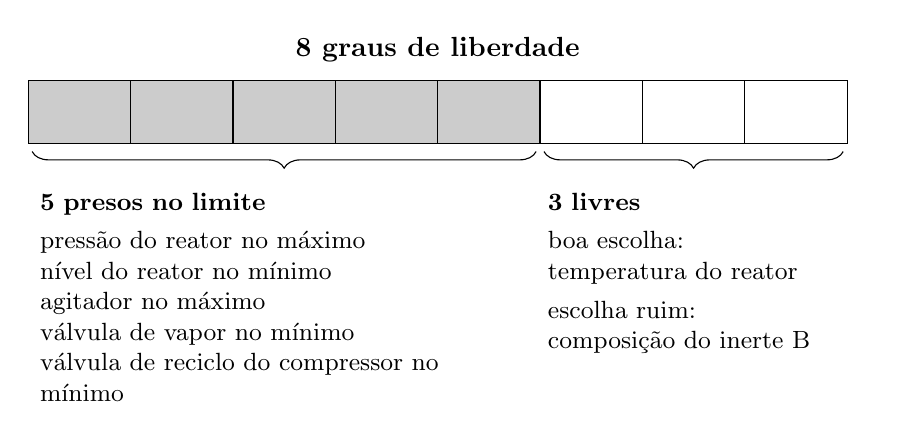
\begin{tikzpicture}[font=\small]
  % 8 graus de liberdade: 5 presos no limite (cinza) e 3 livres (branco)
  \foreach \i in {0,...,4} \draw[fill=black!20] (\i*1.3,0) rectangle ++(1.3,0.8);
  \foreach \i in {5,...,7} \draw (\i*1.3,0) rectangle ++(1.3,0.8);
  \node[font=\bfseries] at (5.2,1.2) {8 graus de liberdade};
  \draw[decorate,decoration={brace,mirror,amplitude=6pt}] (0.05,-0.1) -- (6.45,-0.1);
  \draw[decorate,decoration={brace,mirror,amplitude=6pt}] (6.55,-0.1) -- (10.35,-0.1);
  \node[anchor=north,align=left,text width=6.2cm] at (3.25,-0.5) {%
    \textbf{5 presos no limite}\\[3pt]
    pressão do reator no máximo\\
    nível do reator no mínimo\\
    agitador no máximo\\
    válvula de vapor no mínimo\\
    válvula de reciclo do compressor no mínimo};
  \node[anchor=north,align=left,text width=4.2cm] at (8.7,-0.5) {%
    \textbf{3 livres}\\[3pt]
    boa escolha:\\ temperatura do reator\\[3pt]
    escolha ruim:\\ composição do inerte B};
\end{tikzpicture}
\caption{Graus de liberdade do TEP em regime estacionário no Modo~1.}
\label{fig:graus_liberdade_tep}
\end{figure}

Na hierarquia de Larsson e Skogestad, quem decide e quem executa estão em camadas diferentes. Escolher a temperatura do reator como variável a manter constante é uma decisão de uma camada de cima; quem mantém a temperatura no valor pedido é uma malha da camada regulatória. E saber se essa escolha está funcionando, isto é, se a planta continua perto do custo mínimo depois de um distúrbio, exige medições que vêm da planta e sobem até a camada que decidiu. Ou seja, para que essa estrutura funcione, a informação precisa descer (os setpoints) e subir (as medições e o estado da planta) entre as camadas o tempo todo. Os autores tratam de quais decisões cada camada toma, mas não de como essa informação passa de uma camada para a outra \cite{Larsson2000, Skogestad2004}. Em uma planta real, essas camadas costumam rodar em equipamentos e programas diferentes, então essa passagem não acontece sozinha: alguém precisa construí-la. A Figura~
ef{fig:camadas_integracao} ilustra essa passagem.

É nessa passagem que este trabalho se concentra. Ele é desenvolvido na ênfase de \textbf{Integração de Sistemas de Controle} do curso de Engenharia de Controle e Automação e, por isso, o foco não é escolher as variáveis controladas nem sintonizar controladores, mas construir a ligação entre as camadas: como a planta expõe o seu estado, como esse estado chega a uma camada supervisória e como essa camada registra o que observou. O TEP é usado como a planta sobre a qual essa ligação é montada.

\begin{figure}[htbp]
\centering
\begin{tikzpicture}[
    font=\small,
    bloco/.style={draw, fill=gray!10, minimum width=3.6cm, minimum height=0.85cm, align=center},
    fluxo/.style={-{Latex[length=2mm]}, thick},
    rotulo/.style={font=\scriptsize},
    exemplo/.style={font=\scriptsize, align=left, text width=3.4cm, anchor=west}
]
  % camadas
  \node[bloco] (opt) at (0,0)    {Otimização\[-1pt]\scriptsize (horas)};
  \node[bloco] (sup) at (0,-2.0) {Supervisão\[-1pt]\scriptsize (minutos)};
  \node[bloco] (reg) at (0,-4.0) {Controle regulatório\[-1pt]\scriptsize (segundos)};
  \node[bloco] (tep) at (0,-6.0) {Planta (TEP)};

  % setpoints descem (esquerda), medições sobem (direita)
  \foreach \a/\b in {opt/sup, sup/reg, reg/tep} {
    \draw[fluxo] ([xshift=-0.7cm]\a.south) -- ([xshift=-0.7cm]\b.north)
      node[midway, left, rotulo] {setpoints};
    \draw[fluxo] ([xshift=0.7cm]\b.north) -- ([xshift=0.7cm]\a.south)
      node[midway, right, rotulo] {medições / estado};
  }

  % região de integração
  \draw[dashed, gray!70, rounded corners=2pt] (-2.9,-0.5) rectangle (3.3,-5.5);
  \node[rotulo, rotate=90] at (-3.25,-3.0) {integração (foco deste trabalho)};

  % exemplo
  \node[exemplo] at (3.7,-2.0) {decide manter a temperatura do reator constante};
  \node[exemplo] at (3.7,-4.0) {malha mantém a temperatura no valor pedido};
  \node[exemplo] at (3.7,-6.0) {mede a temperatura e o custo};
\end{tikzpicture}
\caption{Camadas de controle e a informação que passa entre elas.}
\label{fig:camadas_integracao}
\fonte{Elaborado pelo autor a partir de \citeonline{Larsson2000} e \citeonline{Skogestad2004}.}
\end{figure}

A resposta formal a esse problema é o conceito de \textbf{Sistema Cyber-Físico} (CPS): a integração entre computação e processos físicos, onde computadores e redes monitoram e controlam o processo por meio de laços de realimentação em que o físico afeta a computação e vice-versa \cite{Hehenberger2016}. Hehenberger et al.\ apontam que uma abordagem de engenharia baseada em CPS impõe dois passos metodológicos: modelar explicitamente cada subsistema e integrar esses modelos em um sistema global coerente \cite{Hehenberger2016}. A \textit{parte cyber} de um CPS é precisamente a rede de integração — a camada que interconecta subsistemas, torna seus estados visíveis e permite que comandos fluam de volta ao processo. Esse requisito de integração horizontal e vertical é o que torna necessária uma camada de comunicação industrial com semântica padronizada e, consequentemente, motiva as escolhas tecnológicas deste trabalho.


\begin{tikzpicture}[
    >=Latex,
    font=\small,
    bloco/.style={
        draw=black,
        fill=gray!10,
        minimum width=3.8cm,
        minimum height=0.85cm,
        align=center
    },
    fluxo/.style={-{Latex[length=2mm]}, thick},
    exemplo/.style={
        font=\scriptsize,
        align=left,
        text width=3.4cm
    }
]

% Blocos da hierarquia
\node[bloco] (opt) at (0,0)
    {Otimização\\[-1pt]\scriptsize (horas)};

\node[bloco] (sup) at (0,-2.0)
    {Supervisão\\[-1pt]\scriptsize (minutos)};

\node[bloco] (reg) at (0,-4.0)
    {Controle regulatório\\[-1pt]\scriptsize (segundos)};

\node[bloco] (tep) at (0,-6.0)
    {Planta (TEP)};

% Setas descendentes: setpoints
\foreach \a/\b in {opt/sup, sup/reg, reg/tep} {
    \draw[fluxo]
        ([xshift=-0.85cm]\a.south) --
        ([xshift=-0.85cm]\b.north)
        node[midway, left, font=\scriptsize]
        {setpoints};
}

% Setas ascendentes: medições / estado
\foreach \a/\b in {sup/opt, reg/sup, tep/reg} {
    \draw[fluxo]
        ([xshift=0.85cm]\a.north) --
        ([xshift=0.85cm]\b.south)
        node[midway, right, font=\scriptsize]
        {medições / estado};
}

% Região de integração
\draw[
    dashed,
    gray!75,
    rounded corners=2pt
]
    (-2.85,-0.48) rectangle (2.85,-5.52);

\node[
    font=\scriptsize,
    align=center,
    text width=2.5cm,
    anchor=west
] at (3.0,-1.0)
    {integração\\
     (foco deste trabalho)};

% Exemplos por nível
\node[exemplo, anchor=west]
    at (3.0,-2.0)
    {decide manter a temperatura
     do reator constante};

\node[exemplo, anchor=west]
    at (3.0,-4.0)
    {malha mantém a temperatura
     no valor pedido};

\node[exemplo, anchor=west]
    at (3.0,-6.0)
    {mede a temperatura
     e o custo};

\end{tikzpicture}



Para a camada supervisória desse CPS — o componente que observa o estado da planta e age para manter a operação dentro de parâmetros declarados — a literatura cloud-native oferece um candidato bem estudado. Shuiguang et al.\ \cite{Shuiguang2023} caracterizam computação cloud-native como a combinação de microserviços, containerização e orquestração automática de componentes distribuídos, com Kubernetes como o orquestrador open-source que se tornou padrão de fato na indústria. O mecanismo central que o torna atraente para esse papel é o \textit{reconciliation controller loop}: uma comparação contínua entre o estado desejado (\textit{Spec}) e o estado observado (\textit{Status}), seguida de ações para convergir um ao outro \cite{Burns2016}. Essa estrutura — declarar política, observar realidade, reconciliar continuamente — guarda uma semelhança estrutural não trivial com o papel que Skogestad atribui à camada supervisória: manter variáveis controladas em setpoints ótimos usando os graus de liberdade da camada regulatória como alavancas. Este trabalho explora a hipótese de que esse padrão arquitetural pode servir como orquestrador supervisório de um CPS industrial baseado no TEP.

O presente trabalho constrói três artefatos como ponto de partida para esse universo de possibilidades. O primeiro é um microserviço da planta TEP implementado em Rust — uma refatoração do modelo original em FORTRAN para uma linguagem de alta performance, exposto via gRPC. O segundo é uma Interface Homem-Máquina (IHM) web em FastAPI com WebSocket, funcionando como cliente dessa planta e permitindo monitoramento em tempo real e injeção dos distúrbios. O terceiro é um Operator Kubernetes básico que observa a planta, demonstrando a viabilidade de usar o padrão declarativo do Kubernetes como orquestrador supervisório sobre componentes industriais. A interface entre os três componentes é mapeada segundo o padrão OPC~UA, respeitando a norma IEC~62541 \cite{IEC62541_1}. O objetivo não é implementar estratégias de controle nem estabelecer lógica supervisória definitiva — é produzir esses artefatos iniciais como fundação técnica e ponto de partida concreto para os trabalhos futuros que o referencial teórico delineia.

\section{PROBLEMA}
\label{sec:problema}

O problema abordado neste trabalho é a implementação de controle plant-wide sobre o Processo Tennessee Eastman como um desafio de integração industrial. A TEP, com suas unidades interconectadas e laços de reciclo, exige uma camada supervisória que coordene componentes heterogêneos em diferentes escalas de tempo. Para que esse sistema seja extensível e interoperável — e não apenas um protótipo isolado —, seus componentes devem expor interfaces segundo normas industriais estabelecidas, de modo que possam ser compostos, observados e substituídos por ferramentas compatíveis. A abordagem adotada é a de um Sistema Cyber-Físico com Kubernetes como orquestrador supervisório candidato, o que impõe que tanto a planta simulada quanto os demais componentes respeitem uma semântica de integração padronizada.

\section{A PROPOSTA}
\label{sec:proposta}

Este trabalho propõe refatorar o modelo original do TEP de FORTRAN para um microserviço em Rust, modelado segundo a hierarquia de integração da norma IEC~62264 \cite{IEC62264} e com variáveis de processo expostas conforme o padrão OPC~UA \cite{IEC62541_1}. Sobre essa base, são implementados os seguintes componentes:

\begin{enumerate}
  \item Simulação da planta TEP em Rust com integração numérica RK4, comunicação via gRPC e modelagem compatível com a hierarquia Purdue definida pela IEC~62264 \cite{IEC62264};
  \item Interface Homem-Máquina (IHM) web aderente à norma IEC~63303 \cite{IEC63303}, funcionando como cliente da planta para monitoramento em tempo real e injeção de distúrbios;
  \item Implementação dos distúrbios programados descritos no artigo original de Downs e Vogel \cite{DOWNS1993};
  \item Verificação da fidelidade dinâmica da simulação por meio da análise do comportamento da planta sob os distúrbios implementados;
  \item Implementação de um \textit{Custom Resource Definition} (CRD) Kubernetes conectando um contêiner Kind à planta, validando a arquitetura básica do CPS proposto.
\end{enumerate}

\section{OBJETIVOS}
\label{sec:objetivos}

\subsection{Objetivo Geral}

Implementar uma simulação funcional do Processo Tennessee Eastman em Rust — refatoração do modelo original em FORTRAN — e integrá-la em uma arquitetura de Sistema Cyber-Físico com componentes heterogêneos interoperáveis via protocolos abertos, servindo como base técnica para o desenvolvimento futuro de estratégias de controle plant-wide.

\subsection{Objetivos Específicos}
\begin{enumerate}
    \item Verificar que a simulação em Rust reproduz fielmente a dinâmica da planta TEP descrita por Downs e Vogel, por meio da análise do comportamento sob os distúrbios programados do artigo original.
    \item Verificar que a IHM opera corretamente como cliente da planta, respeitando a interface OPC~UA e os requisitos de monitoramento em tempo real definidos pela IEC~63303.
    \item Demonstrar que os componentes heterogêneos do sistema — simulação, IHM e orquestrador — são interoperáveis via a interface padronizada, sem acoplamento direto entre implementações.
    \item Validar que o padrão CRD do Kubernetes consegue observar o estado da planta, estabelecendo a viabilidade arquitetural do Kubernetes como orquestrador supervisório de um CPS industrial.
    \item Estabelecer uma base técnica documentada e reprodutível que permita trabalhos futuros evoluir para estratégias completas de controle plant-wide sobre a mesma infraestrutura.
\end{enumerate}

\section{ORGANIZAÇÃO DO TRABALHO}

Este documento está organizado da seguinte forma. O Capítulo~2 apresenta os fundamentos teóricos: o Processo Tennessee Eastman, os princípios de controle plant-wide, o diagnóstico de qualidade de malhas, a analogia cloud-native, o IEC~61499, o padrão de Operators do Kubernetes, o protocolo gRPC e o OPC UA. O Capítulo~3 descreve o desenvolvimento da infraestrutura proposta, detalhando cada componente e as decisões de arquitetura. O Capítulo~4 apresenta os resultados dos 17 experimentos realizados e a análise do comportamento da planta sob distúrbios. O Capítulo~5 conclui o trabalho e apresenta as direções de trabalhos futuros, incluindo a incorporação de métricas de qualidade de malha à camada supervisória.

Para a camada supervisória desse CPS — o componente que observa o estado da planta e age para manter a operação dentro de parâmetros declarados — a literatura cloud-native oferece um candidato bem estudado. Shuiguang et al.\ \cite{Shuiguang2023} caracterizam computação cloud-native como a combinação de microserviços, containerização e orquestração automática de componentes distribuídos, com Kubernetes como o orquestrador open-source que se tornou padrão de fato na indústria. O mecanismo central que o torna atraente para esse papel é o \textit{reconciliation controller loop}: uma comparação contínua entre o estado desejado (\textit{Spec}) e o estado observado (\textit{Status}), seguida de ações para convergir um ao outro \cite{Burns2016}. Essa estrutura — declarar política, observar realidade, reconciliar continuamente — guarda uma semelhança estrutural não trivial com o papel que Skogestad atribui à camada supervisória: manter variáveis controladas em setpoints ótimos usando os graus de liberdade da camada regulatória como alavancas. Este trabalho explora a hipótese de que esse padrão arquitetural pode servir como orquestrador supervisório de um CPS industrial baseado no TEP.

O presente trabalho constrói três artefatos como ponto de partida para esse universo de possibilidades. O primeiro é um microserviço da planta TEP implementado em Rust — uma refatoração do modelo original em FORTRAN para uma linguagem de alta performance, exposto via gRPC. O segundo é uma Interface Homem-Máquina (IHM) web em FastAPI com WebSocket, funcionando como cliente dessa planta e permitindo monitoramento em tempo real e injeção dos distúrbios. O terceiro é um Operator Kubernetes básico que observa a planta, demonstrando a viabilidade de usar o padrão declarativo do Kubernetes como orquestrador supervisório sobre componentes industriais. A interface entre os três componentes é mapeada segundo o padrão OPC~UA, respeitando a norma IEC~62541 \cite{IEC62541_1}. O objetivo não é implementar estratégias de controle nem estabelecer lógica supervisória definitiva — é produzir esses artefatos iniciais como fundação técnica e ponto de partida concreto para os trabalhos futuros que o referencial teórico delineia.

\section{PROBLEMA}
\label{sec:problema}

O problema abordado neste trabalho é a implementação de controle plant-wide sobre o Processo Tennessee Eastman como um desafio de integração industrial. A TEP, com suas unidades interconectadas e laços de reciclo, exige uma camada supervisória que coordene componentes heterogêneos em diferentes escalas de tempo. Para que esse sistema seja extensível e interoperável — e não apenas um protótipo isolado —, seus componentes devem expor interfaces segundo normas industriais estabelecidas, de modo que possam ser compostos, observados e substituídos por ferramentas compatíveis. A abordagem adotada é a de um Sistema Cyber-Físico com Kubernetes como orquestrador supervisório candidato, o que impõe que tanto a planta simulada quanto os demais componentes respeitem uma semântica de integração padronizada.

\section{A PROPOSTA}
\label{sec:proposta}

Este trabalho propõe refatorar o modelo original do TEP de FORTRAN para um microserviço em Rust, modelado segundo a hierarquia de integração da norma IEC~62264 \cite{IEC62264} e com variáveis de processo expostas conforme o padrão OPC~UA \cite{IEC62541_1}. Sobre essa base, são implementados os seguintes componentes:

\begin{enumerate}
  \item Simulação da planta TEP em Rust com integração numérica RK4, comunicação via gRPC e modelagem compatível com a hierarquia Purdue definida pela IEC~62264 \cite{IEC62264};
  \item Interface Homem-Máquina (IHM) web aderente à norma IEC~63303 \cite{IEC63303}, funcionando como cliente da planta para monitoramento em tempo real e injeção de distúrbios;
  \item Implementação dos distúrbios programados descritos no artigo original de Downs e Vogel \cite{DOWNS1993};
  \item Verificação da fidelidade dinâmica da simulação por meio da análise do comportamento da planta sob os distúrbios implementados;
  \item Implementação de um \textit{Custom Resource Definition} (CRD) Kubernetes conectando um contêiner Kind à planta, validando a arquitetura básica do CPS proposto.
\end{enumerate}

\section{OBJETIVOS}
\label{sec:objetivos}

\subsection{Objetivo Geral}

Implementar uma simulação funcional do Processo Tennessee Eastman em Rust — refatoração do modelo original em FORTRAN — e integrá-la em uma arquitetura de Sistema Cyber-Físico com componentes heterogêneos interoperáveis via protocolos abertos, servindo como base técnica para o desenvolvimento futuro de estratégias de controle plant-wide.

\subsection{Objetivos Específicos}
\begin{enumerate}
    \item Verificar que a simulação em Rust reproduz fielmente a dinâmica da planta TEP descrita por Downs e Vogel, por meio da análise do comportamento sob os distúrbios programados do artigo original.
    \item Verificar que a IHM opera corretamente como cliente da planta, respeitando a interface OPC~UA e os requisitos de monitoramento em tempo real definidos pela IEC~63303.
    \item Demonstrar que os componentes heterogêneos do sistema — simulação, IHM e orquestrador — são interoperáveis via a interface padronizada, sem acoplamento direto entre implementações.
    \item Validar que o padrão CRD do Kubernetes consegue observar o estado da planta, estabelecendo a viabilidade arquitetural do Kubernetes como orquestrador supervisório de um CPS industrial.
    \item Estabelecer uma base técnica documentada e reprodutível que permita trabalhos futuros evoluir para estratégias completas de controle plant-wide sobre a mesma infraestrutura.
\end{enumerate}

\section{ORGANIZAÇÃO DO TRABALHO}

Este documento está organizado da seguinte forma. O Capítulo~2 apresenta os fundamentos teóricos: o Processo Tennessee Eastman, os princípios de controle plant-wide, o diagnóstico de qualidade de malhas, a analogia cloud-native, o IEC~61499, o padrão de Operators do Kubernetes, o protocolo gRPC e o OPC UA. O Capítulo~3 descreve o desenvolvimento da infraestrutura proposta, detalhando cada componente e as decisões de arquitetura. O Capítulo~4 apresenta os resultados dos 17 experimentos realizados e a análise do comportamento da planta sob distúrbios. O Capítulo~5 conclui o trabalho e apresenta as direções de trabalhos futuros, incluindo a incorporação de métricas de qualidade de malha à camada supervisória.
